\documentclass[10pt]{IEEEtran}
\usepackage{preamble}


\begin{document}
\title{Mini-project 1: Tic Tac Toe}

\author{
   Federico Betti, Ivan Bioli\\
  \textit{CS-456 Artificial Neural Networks, EPFL Lausanne, Switzerland}
}


\maketitle

\begin{abstract}
In this report we present the results obtained from training an agent to play Tic-Tac-Toe both against quasi-optimal strategy (up to some user-defined degree of randomness) and by self-practice in an unsupervised fashion, then testing its performance against the optimal strategy and the fully random strategy. In the first section we show the results obtained by tabular Q-Learning, in the second section we show the results from Deep Q-Learning and we compare the two approaches in the last section.
\end{abstract}

\section{Introduction}
\subsection{Notation}
Throughout the report we use the same notation as in the project description, if not stated otherwise.

Moreover, in the following, we define as a \emph{win-booking state} every state in which the current player has the chance to win the game, either with the next move or in two moves with a fork. Two examples of \emph{win-booking state} are provided in \Cref{fig_heatmap_1} and \Cref{fig_heatmap_3}.
%, and similarly a \emph{block-win state} as every state in which the current player must block the chance of winning at the next turn of the adversary \textcolor{red}{in order not to lose the game}. Two examples of a \emph{win-booking state} and of a \emph{block-win state} are provided in \Cref{plot_question_10} a) and b) respectively.

\section{Q-Learning}
Before discussing the results obtained with tabular Q-Learning, we clarify that in this section, in order to reduce the oscillations in the metrics that might occur during a particular training run, we performed 10 complete training runs. This helped us in particular to dump the oscillations which we observed for the measurements of $\mopt$, hence to obtain clearer plots of the training metrics. In all the plots of the current section we show the median over the training runs together, and shaded regions showing the 25 and 75 percentile are possibly shown. \textcolor{red}{Furthermore, in most of the figures of the report, we present only those values of the various parameters which we considered significant and representative of the main trends. We refer to the notebook attached to the submission for the complete results of all the tested values.}

\subsection*{Question 1}
See \Cref{plot_question1}.
\begin{figure}[h]
    \centering
    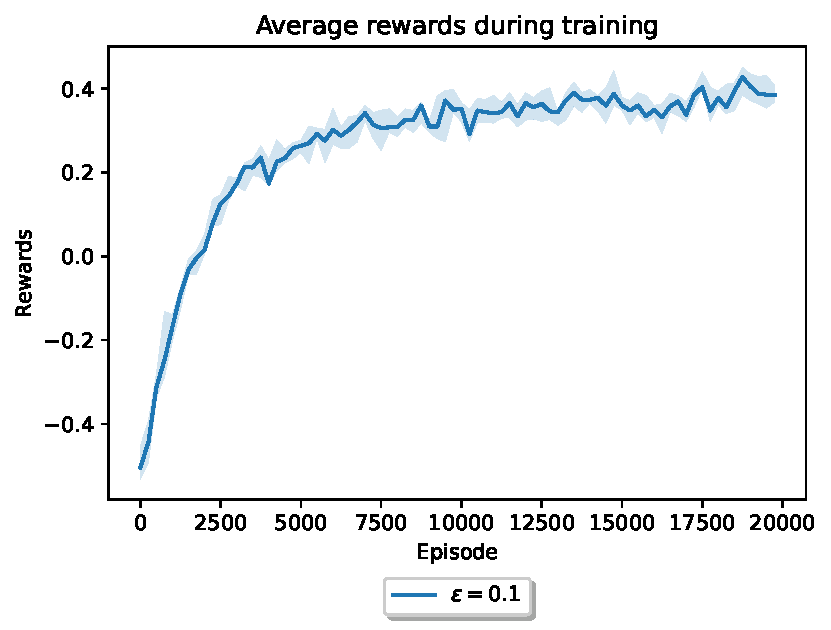
\includegraphics[width = 0.85\linewidth]{code/figures/rewards_epsilon_exploration_Q1.pdf}
    \caption{Training with $\epsilon = 0.1$, an increase in average reward with experience is observed. At the end of training the average reward is positive, indicating that the agent wins more games than it loses against \texttt{Opt(0.5)}. Thus, the agent learns to play Tic-Tac-Toe.}
    \label{plot_question1}
\end{figure}

\subsection*{Question 2  \textcolor{green}{200 words}}
\Cref{plot_question2} shows the average reward during training for different values of $n^{\star}$. It can be observed that using $n^{\star} \gg 1$ initially actions are chosen at random more frequently, therefore the average reward is lower than the one obtained with fixed $\epsilon = \epsmin$. However, when $\epsilon(n)$ reaches $\epsmin$ the average reward approaches the same values observed for fixed exploration rate, with the advantage of a having explored more exhaustively the state space. On the other hand, for very large values of $n^{\star}$ we never reach the constant $\epsmin$-greedy policy, and therefore the average reward attains lower values as the agent keeps paying the price of exploration.

In conclusion, having a decaying exploration rate helps training compared to having a fixed one for values of $n^{\star}$ which guarantee that the agent attains the $\epsmin$-greedy policy towards the end of training: the final average reward is comparable, but with the advantage of a more exhaustive exploration of the state space. On the other hand, having a too high exploration rate throughout the whole training negatively affects the agent's performance.

\begin{figure}[h]
    \centering
    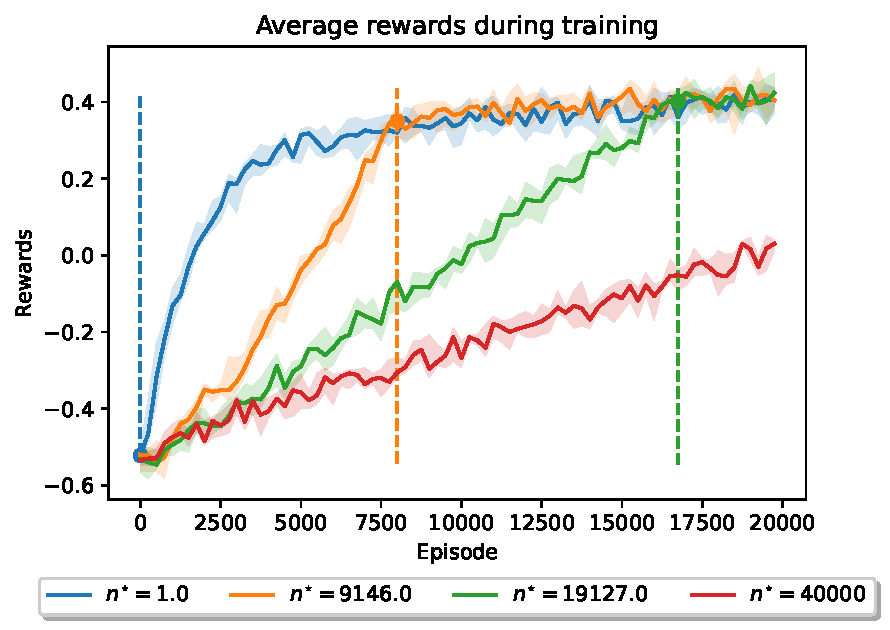
\includegraphics[width = 0.85\linewidth]{code/figures/rewards_n_star.pdf}
    \caption{Average rewards during training against \texttt{Opt(0.5)} for different values of $n^{\star}$: the vertical lines correspond to the episode at which the agent starts choosing moves with the minimum rate of exploration $\epsmin$.}% (for $n^{\star} = 1$ this holds true from the very first episode).}
    \label{plot_question2}
\end{figure}

\subsection*{Question 3  \textcolor{green}{100 words}}
As shown in\Cref{plot_question3}, for all the experimented values $\mopt$ reaches the optimal value $\mopt \ = 0$, with a more gentle growth for higher values of $n^{\star}$ as exploration is more frequent (in expectation) during learning. In general, coherently with the average rewards shown in \emph{Question 2}, higher values of $n^{\star}$ reach their plateau later during training. However, because the performances are an off-policy measure contrarily to the average reward, in this case also $n^{\star} = 40000$ eventually reaches good performances in terms of $\mopt$ and $\mrand$.
\textcolor{red}{Come dire dopo questo che quindi prendiamo 10000?}
%\begin{itemize}
%   \item M opt arrivano tutti a zero ma più o meno steeply perchè viene priorizzata l'exploration
%    \item Soprattutto con 40000 non c'è la grande differenza vista prima perchè prima è la reward è on policy e questo è off-policy.
%    \item Similitudini: salgono a scala e alla fine la performance è comparabile
%    \item Non c'è il flattening (?)
%    \item Dire quale valore scegliamo
%\end{itemize}
\begin{figure}[h]
    \centering
    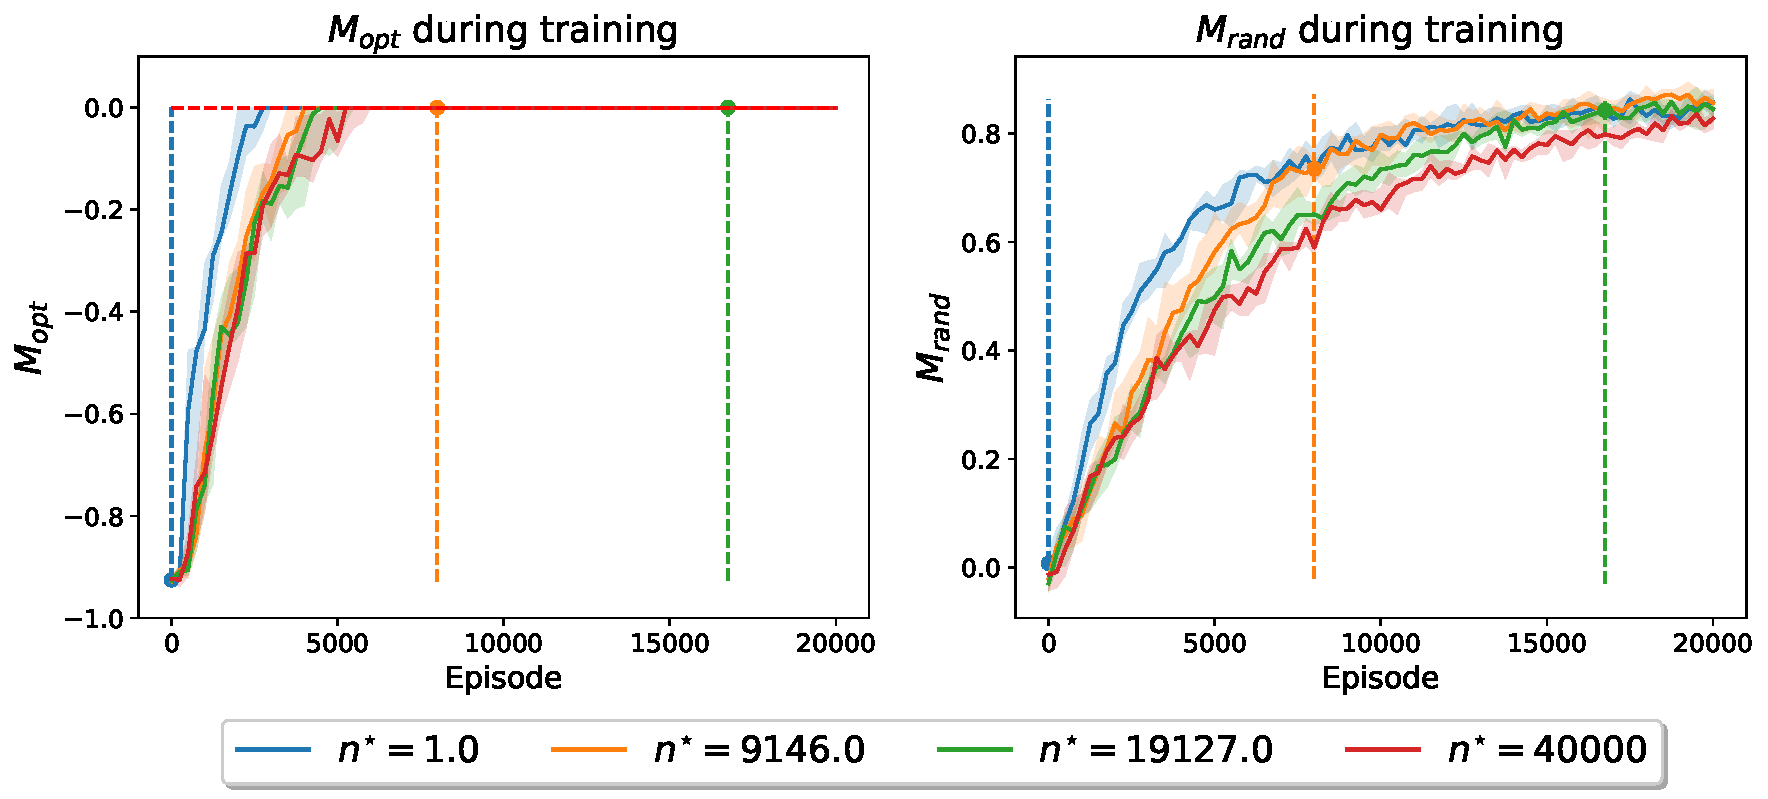
\includegraphics[width=\linewidth]{code/figures/performance_n_star.pdf}
    \caption{Behaviour of \mopt\  and \mrand\  every 250 training episodes for different values of $n^{\star}$.}
    \label{plot_question3}
\end{figure}


\subsection*{Question 4}
As shown in \Cref{plot_question4}, when training against \texttt{Opt(0)} the agent quickly learns to draw against the optimal player, and \mopt\  reaches 0. In contrast, the performance against the random player \mrand\  does not improve significantly because there is no chance of ending up in a \emph{win-booking state}. Hence, all the $Q$-values $Q(s, a)$ with $s$ a \emph{win-booking state} remain equal to their initialization value zero and when the agent plays against the random policy and possibly reaches a \emph{win-booking state}, it chooses the next action randomly, thus a lower \mrand. 

Conversely, when training against \texttt{Opt(1)} \mrand\  quickly increases, while \mopt\  improves slowly without reaching zero. In this case, the agent learns to try to get a $+1$ reward by taking advantage of possible mistakes of his opponent. This implies leaving also to the adversary the chance to win, thus a lower \mopt.
Training against \texttt{Opt(0.5)} both \mopt\  and \mrand\  increase significantly: the agent is able to draw against the optimal policy and to win against the random one. The values $\eopt = 0.2$ and $\eopt = 0.8$ show intermediate results. 

In conclusion, the agent learns to gain optimal rewards (in expectation) against the opponent it is trained against. Indeed the optimal $Q$-values depend on the transition probabilities, which vary with the opponent. If compared with the agent trained against \texttt{Opt(0.5)}, choosing extreme values of $\eopt$ makes the agent gain little in one of the two performance measures and lose much in the other, resulting in a worse general performance.

\begin{figure}[h]
    \centering
    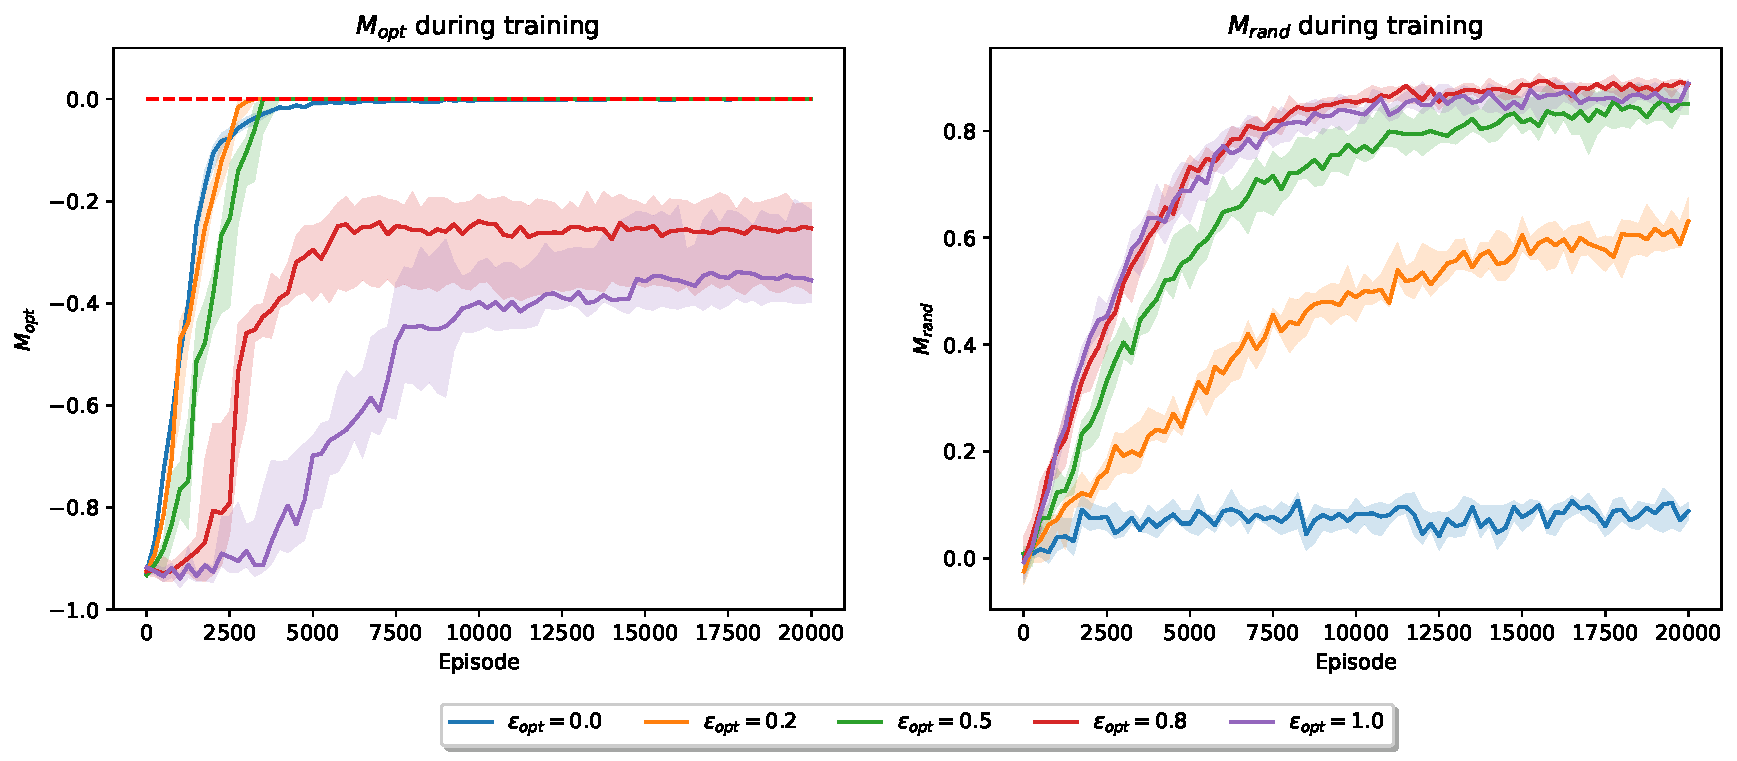
\includegraphics[width=\linewidth]{code/figures/performance_epsilon_opt.pdf}
    \caption{Behaviour of \mopt\  and \mrand\  every 250 training episodes for different values of \eopt.}
    \label{plot_question4}
\end{figure}

\subsection*{Question 5}
The highest values of \mopt\  and \mrand\  training with Q-Learning for $20000$ games against \texttt{Opt($\eopt$)} have been achieved for $\eopt = 0.5$ using decreasing exploration with $n^{\star} = 9146$. They are equal to $\mopt = 0, \, \mrand = 0.85$ (median over 10 runs).

\subsection*{Question 6}
We claim that $Q_1(s,a)$ and $Q_2(s,a)$ do not have the same values, as suggested by \Cref{plot_question4}.
Indeed, the optimal $Q$-values, i.e. those satisfying the Bellman equation, represent the total expected (discounted) reward and depend on the transition probabilities, which are different if playing against \texttt{Opt(0)} or \texttt{Opt(1)}. 

During training, Agent 1 never encounters \emph{win-booking states}, hence at the end of training $Q_1(s,a)$ is equal to the initialization value zero for every \emph{win-booking state} $s$ and every action $a$. This is because the transition probability to any of these states is zero when playing against \texttt{Opt(0)}. Moreover, since Agent 1 can at most draw against \texttt{Opt(0)}, all the rewards are non-positive,  thus also all the Q-values. 

Conversely, Agent 2 encounters \emph{win-booking states} during training and hence we expect $Q_2(s,a) = 1$ (possibly discounted by $\gamma$) for actions that make the agent win. As there exist strictly positive $Q_2(s,a)$, this proves that $Q_2(s,a) \neq Q_1(s,a)$ for some state-action pairs.


\subsection*{Question 7}
\Cref{plot_question7} shows the behaviour of \mopt\ and \mrand\ for different exploration rates $\epsilon$ of the learning agent. We observe that when the agent is trained without any exploration both performance measures are low, as the agent gets stuck performing sub-optimal actions. Increasing the exploration rate $\epsilon$ the performance measures improve and the agent learns to play Tic-Tac-Toe. However, picking a too large exploration rate negatively affects \mopt, while a low one degrades \mrand. The best trade-off between the two metrics is given by $\epsilon = 0.5$.
\begin{figure}[h]
    \centering
    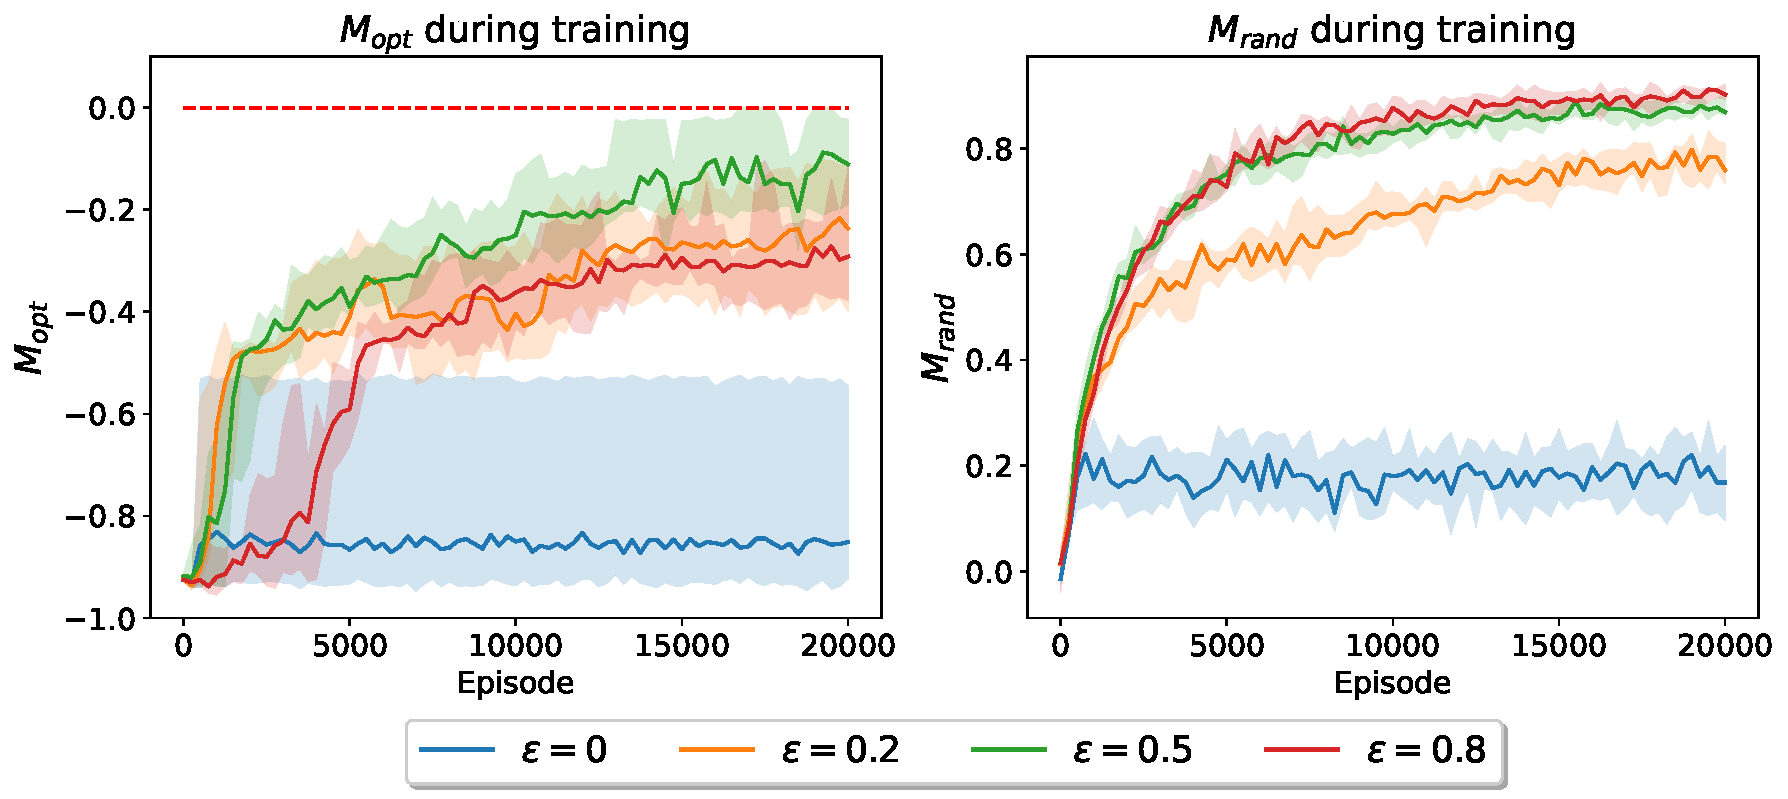
\includegraphics[width=\linewidth]{code/figures/performance_epsilon_self.pdf}
    \caption{Behaviour of \mopt\ and \mrand\ every 250 training episodes for different exploration rates $\epsilon$.}
    \label{plot_question7}
\end{figure}


\subsection*{Question 8  \textcolor{green}{100 words}}
Similarly to \emph{Question 3}, from \Cref{plot_question8} it can be seen that decreasing $\epsilon$ helps training compared to a fixed one if the chosen value of $n^{\star}$ is representative of a well-designed exploration-exploitation trade-off. By prioritizing exploitation during training, i.e. using $n^{\star} = 1$, the agent gets stuck choosing sub-optimal actions. Using larger values of the $n^{\star}$ helps in improving \mrand, but using too high values negatively affects $\mopt$. The best trade-off between the two performance measures is given by $n^{\star} = 24460$.  
%\begin{itemize}
%    \item Mrand cresce bene in scala
%    \item Mopt si intreccia come nella domanda precedente
%    \item nstar aiuta perchè il learning è più veloce e poi si stabilizza.
%    \item Togliere 1000 dal plot.
% \end{itemize}

\begin{figure}[h]
    \centering
    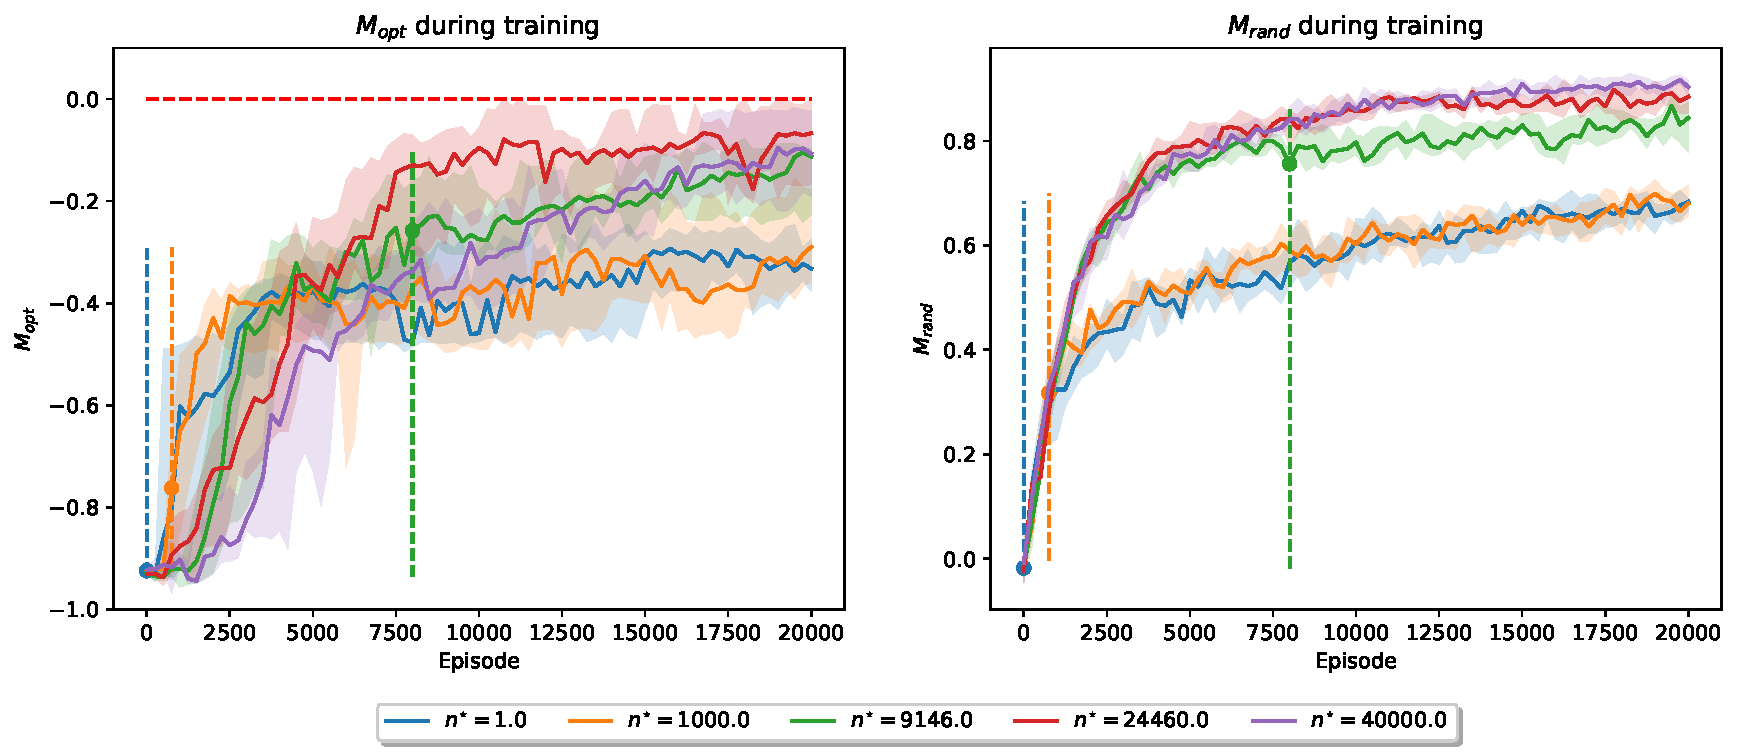
\includegraphics[width=\linewidth]{code/figures/performance_n_star_self.pdf}
    \caption{Behaviour of \mopt\ and \mrand\ over the training episodes for different values of $n^{\star}$.}
    \label{plot_question8}
\end{figure}

\subsection*{Question 9}
The highest values of \mopt\  and \mrand\  training with Q-Learning by self practice for $20000$ games have been achieved using decreasing exploration with $n^{\star} = 24460$ and learning rate $\alpha = 0.05$, and they are equal to $\mopt = -0.07, \, \mrand = 0.87$. However, we noticed that, by picking $\alpha = 0.25$, for the same value of $n^{\star}$ we obtain $\mopt = 0.0, \mrand = 0.93$ (median over 10 runs in both cases).

\subsection*{Question 10  \textcolor{green}{200 words}}
In \Cref{fig_heatmap_1} the highest $Q$-value correctly corresponds to the action that makes the agent (player X) win, but it is not equal to $1$. Furthermore, picking any of the other two empty corners would correspond to a fork, but the estimated $Q$-values are lower than $\gamma = 0.99$. Similarly, in \Cref{fig_heatmap_3} the agent correctly picks the center doing a fork, which brings to victory in one more move, but the Q-value of this action is far from $\gamma$, and the estimates for other win-leading moves such as the south-east corner are even worse. In \Cref{fig_heatmap_2} the agent (player O) correctly blocks the win of the adversary, predicting a negative reward for any other action.

It can be argued that the agent learned the game fairly well, as in the above described scenarios it plays one of the possible correct actions. However, the number of state-action pairs is too high to be sufficiently explored in $20000$ training episodes with tabular Q-Learning, hence the estimated $Q$-values did not converge to their true values, i.e. the ones satisfying the Bellman equation. 

\begin{figure}[h]
     \centering
     \begin{subfigure}[t]{0.32\linewidth}
         \centering
         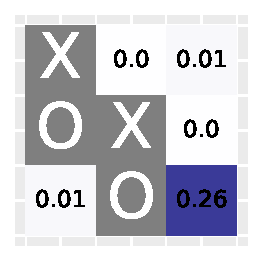
\includegraphics[width=\linewidth]{code/figures/heatmap_0.pdf}
         \caption{Win}
         \label{fig_heatmap_1}
     \end{subfigure}
     \hfill
     \begin{subfigure}[t]{0.32\linewidth}
         \centering
         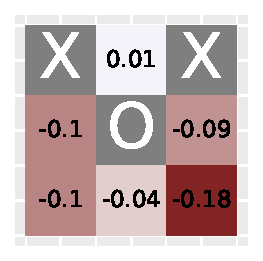
\includegraphics[width=\linewidth]{code/figures/heatmap_1.pdf}
         \caption{Block-win}
         \label{fig_heatmap_2}
     \end{subfigure}
     \hfill
     \begin{subfigure}[t]{0.32\linewidth}
         \centering
         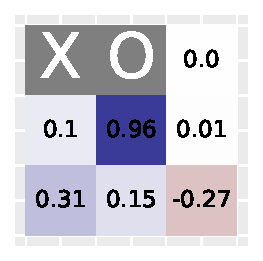
\includegraphics[width=\linewidth]{code/figures/heatmap_2.pdf}
         \caption{Fork}
         \label{fig_heatmap_3}
     \end{subfigure}
        \caption{$Q$-values of available actions in three different board arrangements. The player moving first is always X.}
        \label{plot_question_10}
\end{figure}

\section{Deep Q-Learning}
Similarly to the previous section, also for Deep Q-Learning experiments we average over multiple training runs. The plots show the median over 4 training runs together with the 25 and 75 percentiles. Moreover, also in this section we show in the plots only those values of the parameters which were representative of the main trends, referring to the notebook attached in the submission for the complete results of all the tested values. 

We fine tuned the learning rate and from a grid search the optimal valued turned out to be $\alpha = 10^{-4}$ for both the learning by experts and the learning by self-practice.

\subsection*{Question 11 \textcolor{green}{50 words}}
See \Cref{plot_question11}.
\begin{figure}[h]
    \centering
    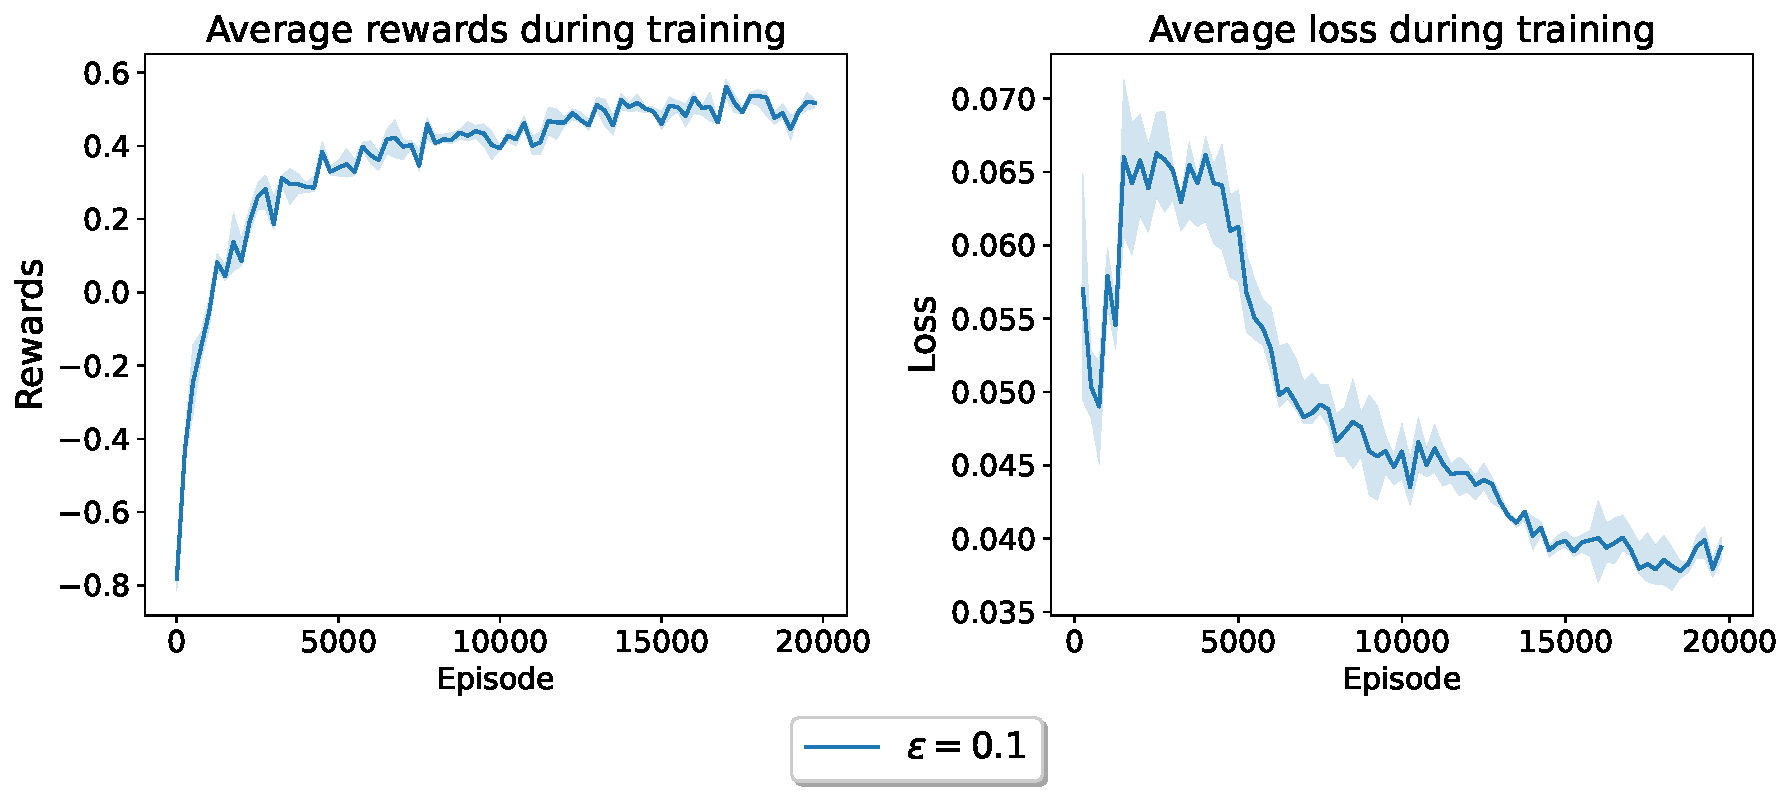
\includegraphics[width = \linewidth]{code/figures/rewards_epsilon_exploration_Q11.pdf}
    \caption{Training with $\epsilon = 0.1$, the loss initially increases, but it flattens when the replay buffer is filled up and then decreases. The reward is initially negative as the agent chooses unavailable actions, but it increases with experience and becomes positive, indicating that the agent learns to play Tic-Tac-Toe.}
    \label{plot_question11}
\end{figure}

\subsection*{Question 12 \textcolor{red}{50 words}}
See \Cref{plot_question12}. 
\begin{figure}[h]
    \centering
    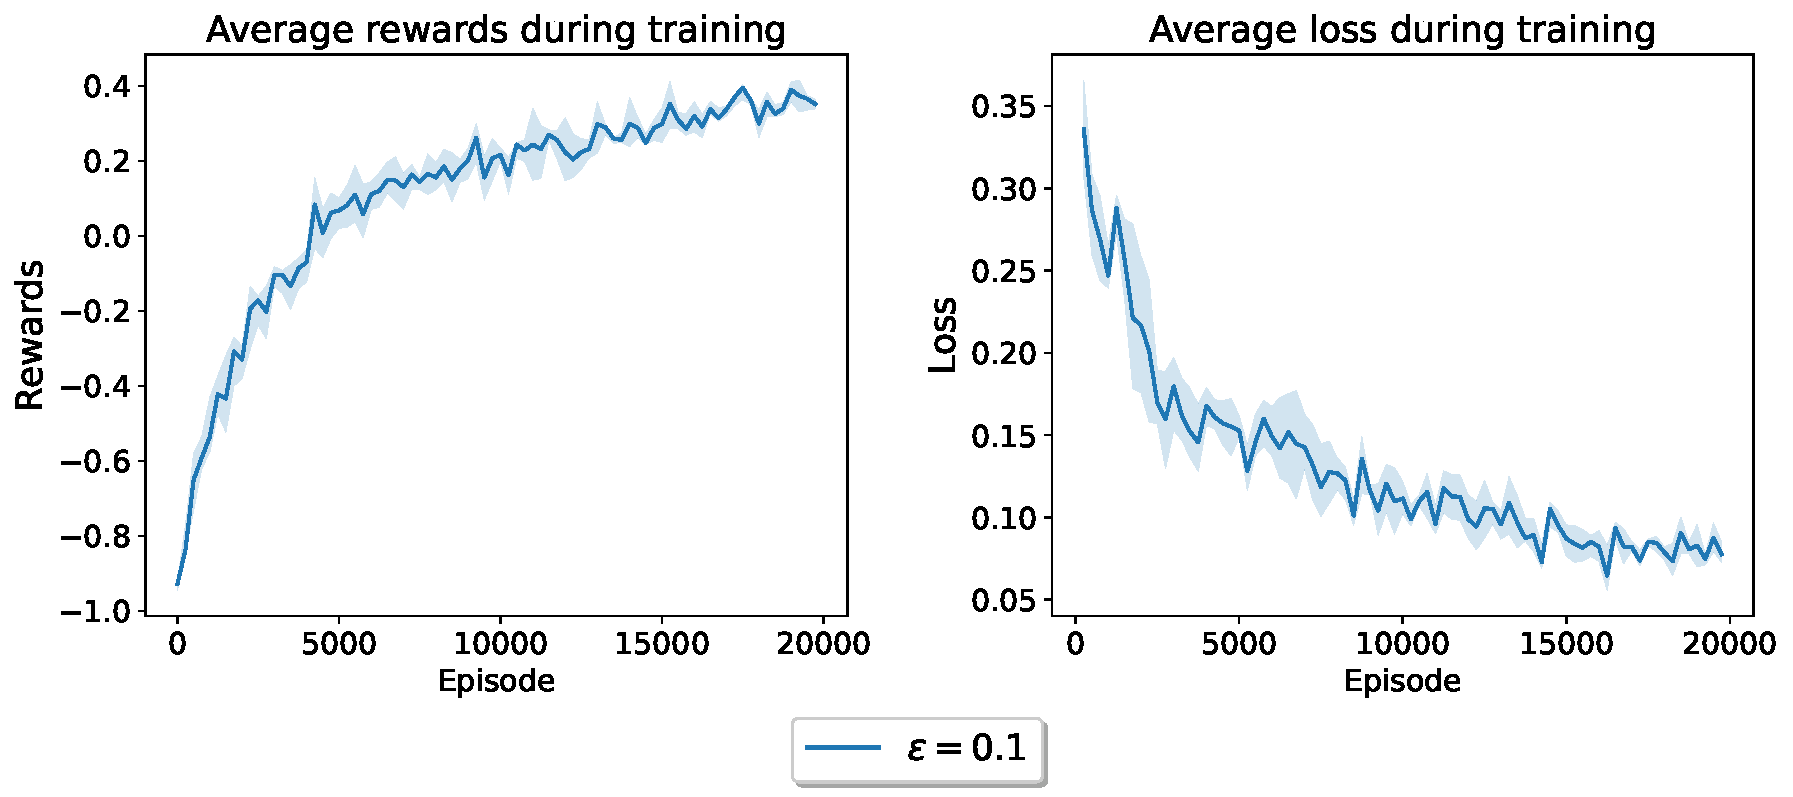
\includegraphics[width = \linewidth]{code/figures/rewards_epsilon_exploration_Q12.pdf}
    \caption{Training with $\epsilon = 0.1$ and  using only the latest transition, the loss is significantly higher than in \Cref{plot_question11} and decreases from the beginning, as the buffer is immediately full. Moreover, the reward increases less steeply and attains a lower value. Hence using a replay buffer and a larger batch-size helps training.}
    \label{plot_question12}
\end{figure}

\subsection*{Question 13  \textcolor{green}{250 words}}
\Cref{plot_question13} shows the effect of the exploration decay rate $n^{\star}$ on the performance measures \mopt\  and \mrand.
It can be seen that for $n^{\star} = 1$, i.e. constant rate of exploration $\epsilon = \epsmin$, \mopt\ increases rapidly in the initial stages of training. On the other hand, the higher the value of $n^{\star}$, the slower the convergence of \mopt\ to the optimal value $\mopt = 0$. 
For all the experimented values of $n^{\star}$ the performance measure \mrand\ rapidly grows above the value $\mrand = 0$, i.e. the agent learns the rules of the game and stops choosing unavailable actions. When using $n^{\star} = 1$ \mrand\ has a more gentle growth and flattens after reaching a sub-optimal plateau. Using larger values of $n^{\star} \gg 1$ helps in achieving a higher \mrand, with a comparable final performance for all values shown in the plot.
Furthermore, in the initial stages of training the metrics \mopt\ and \mrand\ show larger oscillations for higher values of $n^{\star}$, due to a greater rate of random moves.

In conclusion, using a decreasing exploration rate $\epsilon$ helps compared to a fixed rate $\epsilon = \epsmin$, which results in a lower final value of \mrand. However, choosing $n^{\star}$ too high, e.g. $n^{\star} = 40000$, increases the training variance and does not provide benefits in terms of the performance measures \mopt\ and \mrand. Intermediate values of $n^{\star}$, in our case $n^{\star}=10000,\,20000$, are the ones providing the better trade-off between exploration and exploitation. Thus for the following question we choose $n^{\star} = 20000$.

\begin{figure}[h]
    \centering
    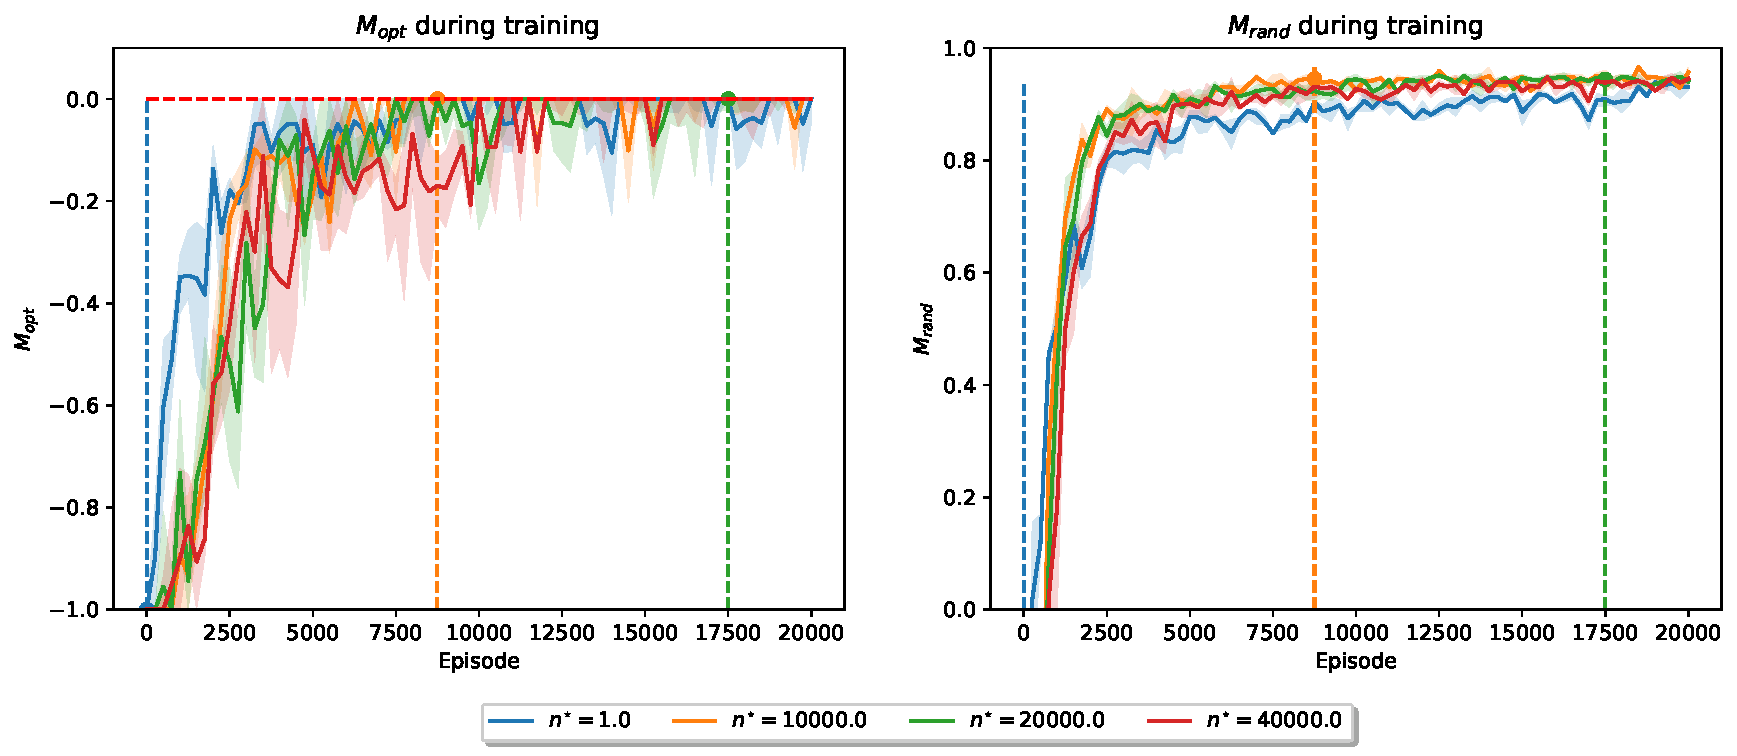
\includegraphics[width = \linewidth]{code/figures/performance_dqn_n_star.pdf}
    \caption{\emph{Question 13}: behaviour of \mopt\  and \mrand\  every 250 training episodes for different values of $n^{\star}$.}
    \label{plot_question13}
\end{figure}
\subsection*{Question 14 \textcolor{green}{250 words}}
As shown in \Cref{plot_question14}, training with $\eopt = 0$ the agent quickly learns to draw against the optimal player and \mopt \ stabilizes at $0$ in the early stages of training. Conversely, the performance against the random player \mrand\  does not improve significantly and remains below zero. Indeed \texttt{Opt(0)} has a deterministic policy, thus when training against it there is no chance of visiting some of the possible states, such as \emph{win-booking states}. When, during testing, the agent plays against the random policy and possibly reaches one of these states, it chooses the next move almost randomly and might even choose one of the unavailable actions, thus the negative average reward. 

Increasing $\eopt$, \mrand\ significantly improves for all values of \eopt, with a slightly more gentle growth for smaller values of \eopt. However, increasing it too much makes learning unstable and degrades the performance measure \mopt. Indeed, for the extreme case $\eopt = 1$, the agent learns to try to get a $+1$ rewards by taking advantage of possible wrong moves of the adversary. This implies exposing itself to the risk of losing the game: while the chance is frequently not taken by the random player during training, it negatively affects \mopt\ when testing. 

Coherently with the results of \emph{Question 4}, it can be argued that when learning by experts the agent learns to gain optimal rewards against the opponent it is trained against, as the transition probabilities depend on the opponent. The best trade-off between the two performance measures is obtained for $\eopt$ around $0.5$. 
\begin{figure}[h]
    \centering
    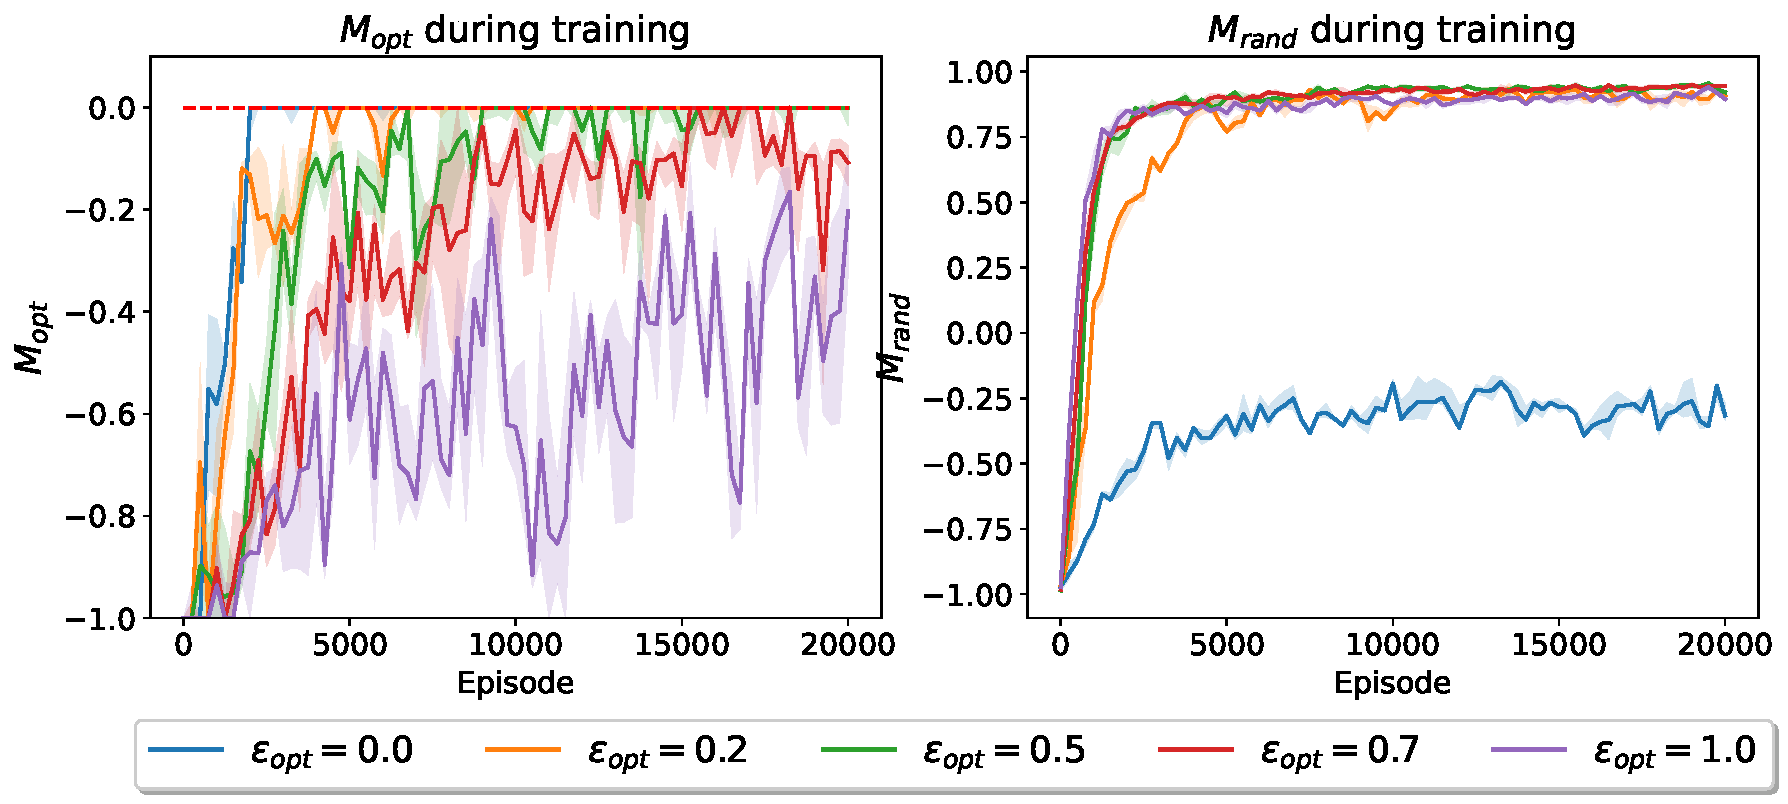
\includegraphics[width = \linewidth]{code/figures/performance_dqn_epsilon_opt_experts.pdf}
    \caption{Behaviour of \mopt\  and \mrand\ for different values of $\eopt$ and $n^{\star} = 20000$.}
    \label{plot_question14}
\end{figure}

\subsection*{Question 15}
The highest values of \mopt\  and \mrand\  training with DQN for $20000$ games against \texttt{Opt($\eopt$)} have been achieved for $\eopt = 0.5$, using decreasing exploration with $n^{\star} = 20000$ and learning rate $\alpha = 10^{-4}$. They are equal to $\mopt = 0, \, \mrand = 0.94$ (median over $4$ runs).

\subsection*{Question 16 \textcolor{green}{100 words}}
\Cref{plot_question16} shows that for $\epsilon = 0$, i.e. greedy policy, the agent does not learn to play as it gets stuck playing sub-optimal actions. On the contrary, taking $\epsilon > 0$ both \mopt\ and \mrand\ significantly increase during training and the agent learns to play Tic-Tac-Toe. Coherently with the results of \emph{Question 7}, too high values of $\epsilon$ lead to a worse performance against the optimal player, while too low values result in a less sharp increase of \mrand. 
%As expected since we are training the agent by playing against itself, this trend is similar to the one obtained when training against \texttt{Opt($\eopt$)} for different values of $\eopt$. 
Thus, the best trade-off between the two performance measures was obtained with $\epsilon = 0.5$.
\begin{figure}[h]
    \centering
    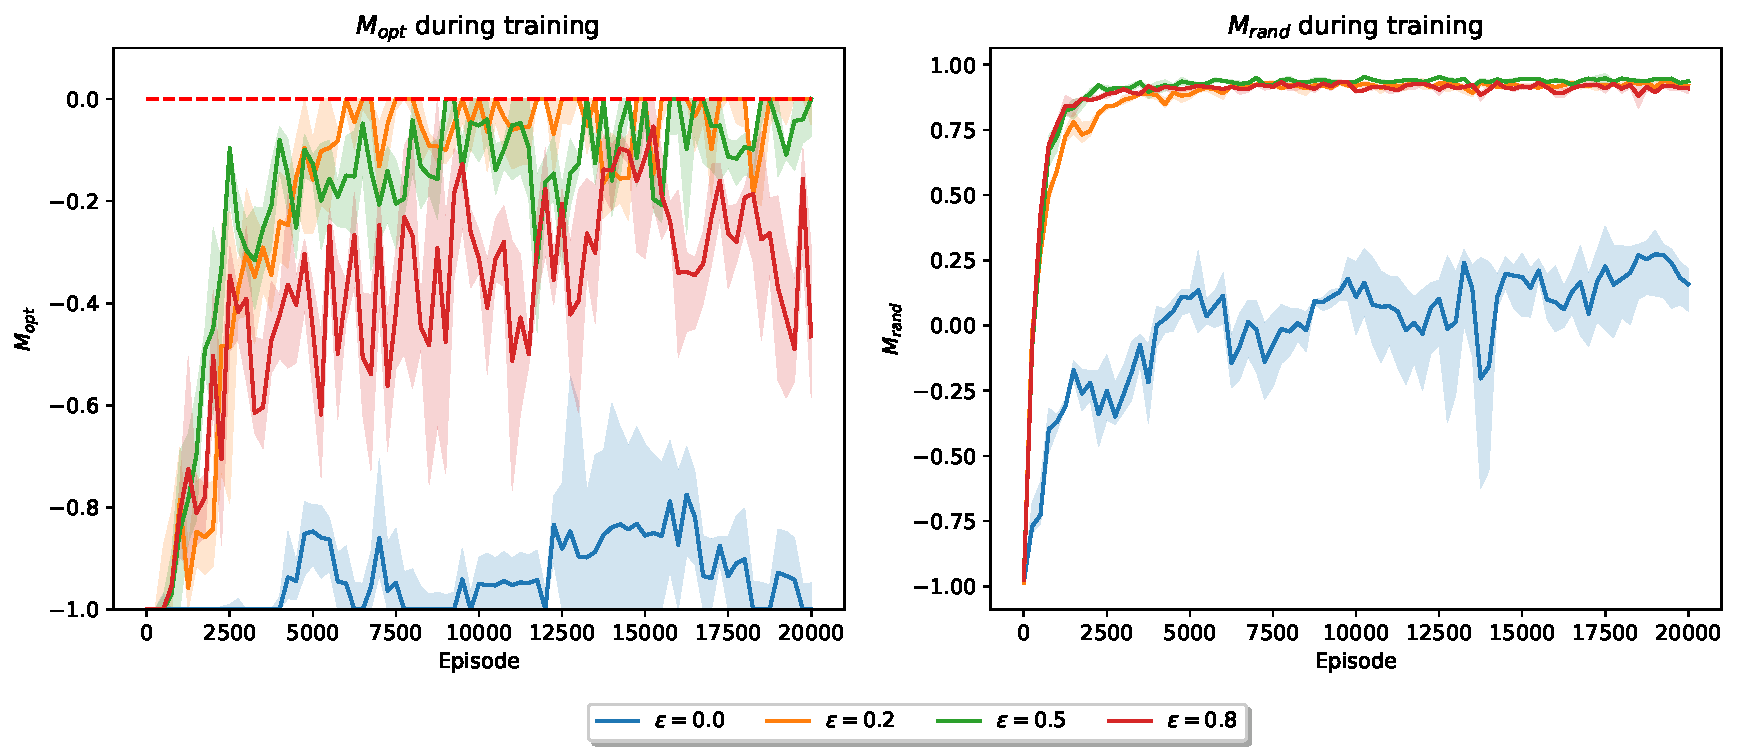
\includegraphics[width = \linewidth]{code/figures/performance_epsilon_dqn_self.pdf}
    \caption{Behaviour of \mopt\ and \mrand\ for different values of the exploration rate $\epsilon$.}
    \label{plot_question16}
\end{figure}
\subsection*{Question 17  \textcolor{green}{100 words}}
\Cref{plot_question17} shows that all values of the decaying exploration rate have similar performances, reaching the optimal value $\mopt = 0$ towards the end of training. On the other hand, choosing constant rate of exploration $\epsilon = \epsmin$, \mrand \ flattens at a sub-optimal level. Hence using a decreasing $\epsilon$ helps training. However, a too high exploration rate, e.g. using $n^{\star} = 40000$, results in more oscillating values of \mopt. The best trade-off between exploration and exploitation was given by $n^{\star} = 10000$.    
\begin{figure}[h]
    \centering
    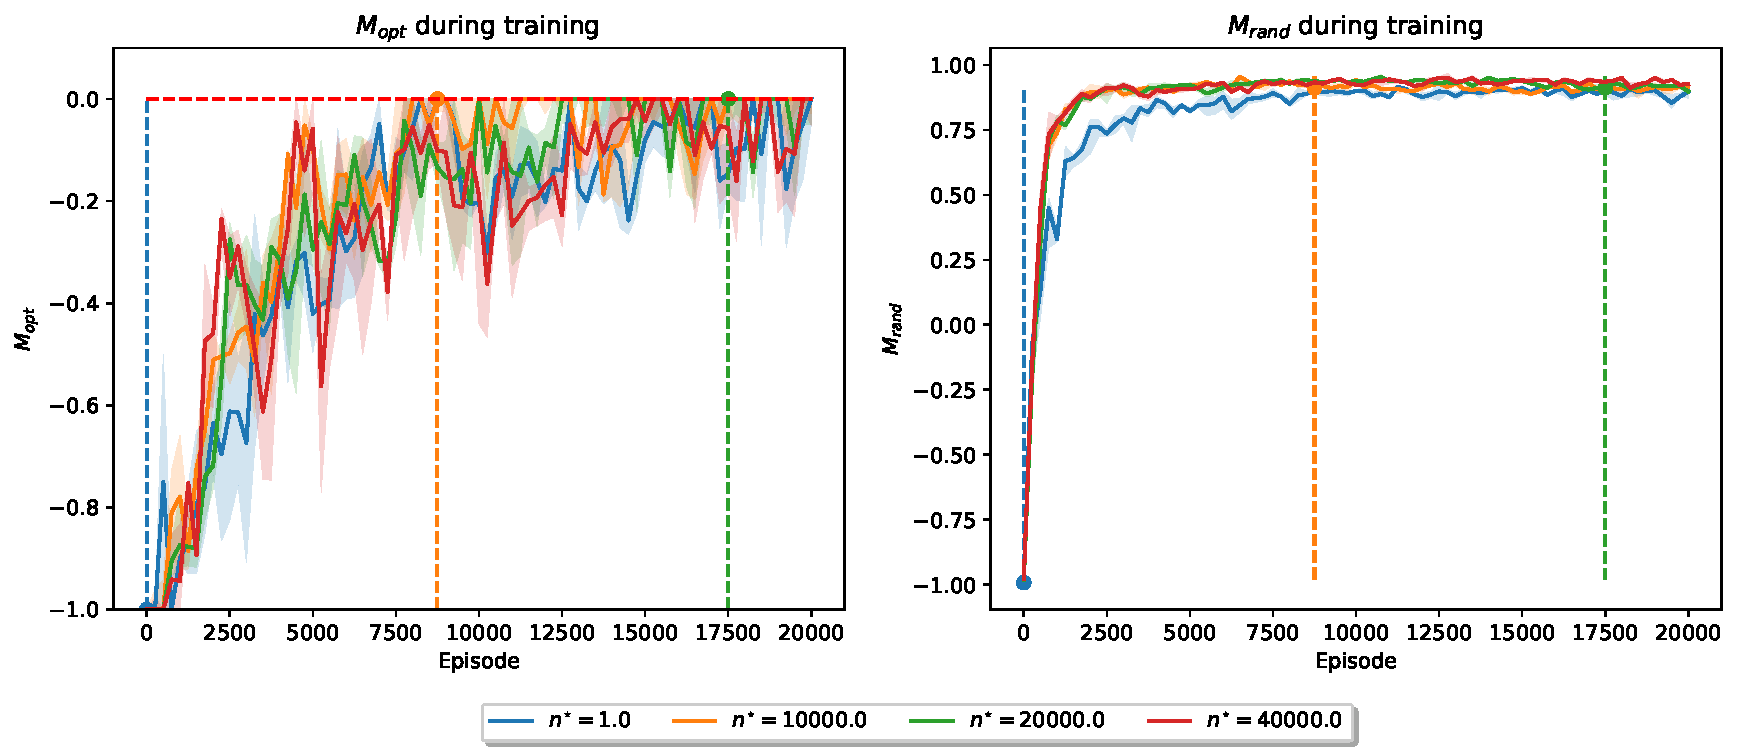
\includegraphics[width = \linewidth]{code/figures/performance_n_star_dqn_self.pdf}
    \caption{Behaviour of \mopt\ and \mrand\ for different values of $n^{\star}$: the vertical lines correspond to the episode at which the agent starts choosing moves with the minimum rate of exploration $\epsmin$.}
    \label{plot_question17}
\end{figure}

\subsection*{Question 18}
The highest values of \mopt\  and \mrand\  training with DQN by self practice for $20000$ games have been achieved using decreasing exploration with $n^{\star} = 10000$ and learning rate $\alpha = 10^{-4}$, and they are equal to $\mopt = 0, \, \mrand = 0.91$ (median over $4$ runs).

\subsection*{Question 19  \textcolor{green}{200 words}}
In \Cref{fig_deep_heatmap_1}, the highest $Q$-value correctly corresponds to the move that makes the agent (player X) win, but it is higher than the reward $r = +1$. Moreover, playing in any of the other two empty corners corresponds to a fork, thus the related $Q$-values are correctly positive, even if not equal to the optimal value $\gamma$. In \Cref{fig_deep_heatmap_2} the agent (player O) blocks the opponent's win and predicts a strongly negative reward for all other actions. Finally, in \Cref{fig_deep_heatmap_3} the agent (player X) correctly picks one of the two possible fork moves, and both have a $Q$-value close to one.

In conclusion, it can be argued that the agent learned the game well: in the above described board arrangements, the agent picks one of the possible correct actions and the $Q$-values do make sense. However, as expected since we are using a neural network to approximate the $Q$-values, the $Q$-values do not exactly match the optimal ones and in particular they do not range in the interval $[-1,1]$.

\begin{figure}[h]
     \centering
     \begin{subfigure}[t]{0.32\linewidth}
         \centering
         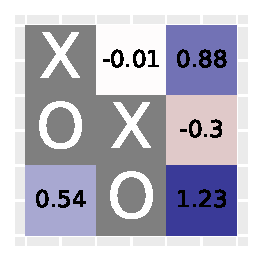
\includegraphics[width=\linewidth]{code/figures/deep_heatmap_0.pdf}
         \caption{Win}
         \label{fig_deep_heatmap_1}
     \end{subfigure}
     \hfill
     \begin{subfigure}[t]{0.32\linewidth}
         \centering
         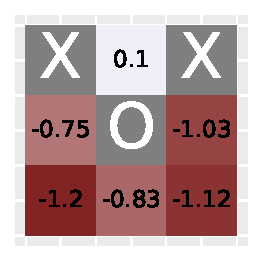
\includegraphics[width=\linewidth]{code/figures/deep_heatmap_1.pdf}
         \caption{Block-win}
         \label{fig_deep_heatmap_2}
     \end{subfigure}
     \hfill
     \begin{subfigure}[t]{0.32\linewidth}
         \centering
         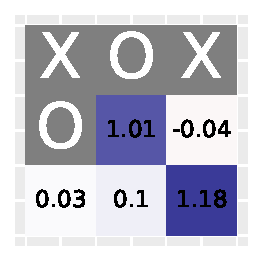
\includegraphics[width=\linewidth]{code/figures/deep_heatmap_2.pdf}
         \caption{Fork}
         \label{fig_deep_heatmap_3}
     \end{subfigure}
        \caption{$Q$-values of available actions in three different board arrangements. The player moving first is always X.}
        \label{plot_question9}
\end{figure}
\section{Comparing Q-Learning with Deep Q-Learning}
\subsection*{Question 20}
\begin{table}[h]
\center
\begin{tabular}{llll}
\hline
 Learning algorithm & \mopt & \mrand & $T_{\mathrm{train}}$ \\
 \hline
 Q-Learning by experts&  0.00 & 0.85 & 6625 \\
 Q-Learning self-practice& -0.07 & 0.87 & 6625 \\
 DQN by experts& 0.00 & 0.94 & 3500 \\
 DQN self-practice& 0.00 & 0.91 & 4000 \\
  \hline 
\end{tabular}
\label{tab_performance}
\caption{Best performance and corresponding training time for $Q$-Learning (median over 10 runs) and DQN (median over 4 runs).}
\end{table}
\subsection*{Question 21  \textcolor{red}{300 words}}
However, DQN provides the greatest advantages when learning by self-practice.

Moreover, as shown in \emph{Question 11-12}, using a replay buffer allows to reduce the sample complexity. Even if in our case interactions with the environment are not expensive, this shows another potential advantage of DQN over tabular Q-Learning.

In conclusion, it can be argued that since the state space is discrete but contains a too high number of state-action pairs to be exhaustively explored in 20000 games, modelling Q-values by a neural networks and learning the weights, such as in DQN, allows to have a faster and more reliable learning if compared to tabular Q-Learning.

\nocite{*}
\printbibliography

\clearpage
\detailtexcount{main}

\end{document}